
\iffalse
In future will rewrite such that KL is obeyed
But as a thought experiment, if the number of samples goes to infinity, shouldn't the distance metric between the datasets generated from the physical process go to 0?
\fi

\begin{abstract}
We demonstrate a proof of principle for using a normalizing flow to learn a physics process's probability distribution to effectively sample more data. In this work, we used traditional physics simulations to generate a dataset $\mathbf{x}$ of 5 million data points with each data point having 4 features.  We take as input a constant 4D normal distribution $p(\mathbf{z})$ , and examine whether the flow model can learn the transformation to $p(\mathbf{x})$ using a random subset of $\mathbf{x}$ for training. We observed a reasonable agreement between the given physics sample and the newly-sampled data using the flow model both in visualization and quantified the metrics.
\end{abstract}
\section{Introduction including Related Works }
%(we can now cite Stan's work! \textcolor{red}{did he already submit his thesis to DSpace MIT?})

Large scale particle physics experiments use humankind's largest machines to study nature at the smallest scales. One such experiment, called CLAS12 in Virginia at the Thomas Jefferson National Accelerator Facility (JLab) (\citet{BURKERT2020163419}), collides ultrarelativistic electrons moving only 1 m/s slower than the speed of light into an ultracold bunch of hydrogen to glean information about the substructure of the proton. In particular, two photons, one electron and one proton in the final state is known as Deeply Virtual $\pi^0$ Production (DV$\pi^0$P), and this process is currently under detailed study as its properties are related to the mechanical properties of the proton (\citet{PhysRevD.55.7114}).

The standard technique to validate experimental particle physics results is to compare real data to the output of detailed experimental simulations, wherein Monte-Carlo (MC) methods are used to walk simulated particles through a detector system in many small time steps (\citet{PhysRevLett.115.212003, 10.1093/ptep/ptaa104}). This microphysics processing begins with field-theoretic functions and empirical physics models, and swims each particle iteratively through a model geometry, solving matrices of force equations at every step. This simulation, typically performed using the GEANT4 package (\citet{AGOSTINELLI2003250}), is very computationally expensive: processing the optimal number of physics events (10,000) on a single core takes 5 hours. 

Our real physics experiment will produce about 10M events, and with the common expectation of a factor of 10 more simulation data compared to real data, we will need 100M simulated physics events, which would consume 50,000 core-hours. Thus, we stand to save a huge amount of processing time if we can train a model on the distribution generated by only several million microphysics generated datapoints, and sample the rest from the trained model. Several groups in particle physics are trying to develop similar methods, for example, training flows to reduce LHC simulation time (\citet{stan}) or work at MIT's IAIFI focused on speeding up aspects of Lattice QCD by a factor of up to 1,000 (\citet{phialia}). 


The normalizing flow is an effective model to learn a probability distribution $p(x)$ when a sample data set $X=\{x\}$ following the distribution is given. The basic idea is a series of transformation $g_i$'s, which are referred to as flows, transforms a prior probability $p(z)$ distributions into the target distribution $p(x)$. That is
\begin{align}
    \mathbf{x} =& g_N \circ g_{N-1}\circ ... \circ g_1 (\mathbf{z}) \\
    \mathbf{z} =& f_1 \circ ... \circ f_{N-1} \circ f_N (\mathbf{x}) \label{eqn:invertible}
\end{align}
, where $f_{N-i+1}\equiv g_i^{-1}$ following \citet{9089305}'s convention. Both $\mathbf{x}$ and $\mathbf{z}$ are vectors of the same dimension $d$. From the eq.~\ref{eqn:invertible}, $g_i$ requires an invertibility condition. An intermediate flow $\mathbf{z_i}$ is defined as follows.
\begin{align}
\mathbf{z_i} =&g_i \circ ... \circ g_1(\mathbf{z}) \label{eqn:forward}\\
    =&f_{i+1}\circ ...f_N(\mathbf{x}) \label{eqn:backward}
\end{align}
, where the flow is expressed in forward direction at eq.~\ref{eqn:forward}, and in backward direction at eq.~\ref{eqn:backward}. Therefore, $\mathbf{z_{i+1}}=g_i (\mathbf{z_i})$ and $\mathbf{z_i} = f_{N-i+1}(\mathbf{z_{i+1}})$ for one flow, or layer. If the $f_i$'s are differentiable, the PDF evolves as follows.
\begin{align}
 p(\mathbf{z_{i+1}})=& p(\mathbf{z_i})|\frac{\partial f_{N-i+1}}{\partial \mathbf{z_i}}| =p(\mathbf{z_i})|\frac{\partial g_{i}^{-1}}{\partial \mathbf{z_i}}|\\
 \log p(\mathbf{z_{i+1}}) =& \log p(\mathbf{z_i}) + \log|\frac{\partial g_i^{-1}}{\partial \mathbf{z_i}}| \label{eqn:logprob}\\
 \log p(\mathbf{x}) =& \log p(\mathbf{z}) + \sum\limits_{i=1}^N \log|\frac{\partial g_i^{-1}}{\partial \mathbf{z_i}}|.
\end{align}
Eq.~\ref{eqn:logprob} is useful to define the forward and the backward propagation of each layer.
Once the NF model is trained to learn the distribution $g: p(z)\rightarrow p(x)$, it is possible to sample $x$ using sampled $z$. \citet{PhysRevD.101.076002} showed that the Nonlinear Independent Component Estimation (NICE) (\citet{Dinh15}) implementation of NF performs well by comparing the technique to existing methods in terms of efficiencies that are defined as average weight during the generation.

Motivated by \citet{stan}'s work, we use Masked Autoregressive Flows (MAF, \citet{papamakarios2018masked}), which is one of the generalized versions of NICE. The MAF starts from a simple fact that $p(z_{i}) = \prod\limits_{j}p(z_{i,j}|\mathbf{z}_{i,0:j-1})$. The component $z_{i,j}$ is the $j$-th component of $z_i$, and the vector $\mathbf{z}_{i,0:j-1}$ is defined as $\{z_{i, 0}, ..., z_{i, j-1}\}$. The transformation is finally defined as
\begin{align}
    z_{i+1, j}=& \sigma_{i, j} z_{i, j} + \mu_{i+1, j}.
\end{align}
The moments $\mu_{i+1, j}$ and $\sigma_{i, j}$ are the mean and standard deviation of $p(z_{i+1,j}|\mathbf{z}_{i+1,0:j-1})$ ($\equiv p(z_{i+1,0})$ for $j=0$). We train the flows to learn $\mu_{i+1, j}$'s and $\sigma_{i, j}$'s, and sample $p(\mathbf{x})$.

\citet{papamakarios2018masked} presents a good github repository of how to train a NF for a 2-dimensional distribution. The libraries are very straightforward and use PyTorch. The architecture consists of the two layers of MAF and the 2D normal prior distribution.
\section{Methods}
%We should include our work of generating the data (GEMC) and processing the data (convert to root, pandas, pickle) as these are all non-trivial steps and a good "data pipeline"
The set of 5M data points were created by using the Open Science Grid (OSG) to process 2,500 core-hours of simulations. The original data format is in ROOT \cite{root}, which is a widely-used format in high energy physics written in C++. There have been improvements in python libraries like uproot \cite{uproot} that can interpret the ROOT data format. The data file has been read using uproot, and saved in pickle, a standard Python library for serializing data \footnote{\url{https://github.com/6862-2021SP-team3/hipo2pickle}}. The pickled data has 5M row, each of which contains the features of four individual particles. Each individual particle has 3 features (magnitude of momentum, polar angle, azimuthal angle), but at this point in our project, we only are able to yield reasonable results using the momenta of all four particles, thus $\mathbf{x}$ has dimensions of $5\text{M}\times4$. Our physics data set also includes $\mathbf{z}$ of the same dimensions as $\mathbf{x}$, but as sampled data points, not in the analytic distributions. This report only utilizes training from $\mathbf{x}$, with the utility of $\mathbf{z}$  being currently investigated.


A normalizing flow template repository was used as a base for our project; we modified the libraries as needed to suite our purpose \footnote{\url{https://github.com/6862-2021SP-team3/nflows/blob/master/nflow.ipynb}}. After many trials of different combinations of hyper parameters, we found an effective training method to being with a 4D normal distribution, use 10 layers of MAF with 16 hidden variables per layer, and train the model with between 200 - 2,000 iterations. Each iteration used randomly sampled training data sets of $1\text{k}\times$4 dimension from the 5M data points generated by physics simulations. To evaluate our model, we sampled 100k data points, $\mathbf{x_1}$, from the physics simulation set which were not included in training, and generated 100k data points, $\mathbf{x_2}$, using our trained model.The KL Divergence (KLD, \citet{Kullback51klDivergence}) and the Earth Mover's Distance (EMD), also known as the Wasserstein-1 Distance (\citet{Dobrushin} were calculated between $\mathbf{x_1}$ and $\mathbf{x_2}$. Since our sample data size was somewhat small, we sampled a second set of 100k data points, $\mathbf{x_1'}$, from the physics simulation set, and calculated KLD and EMD values between  $\mathbf{x_1}$ and $\mathbf{x_1'}$, to have a benchmark to compare with the metrics from the normalized flow comparison.

\section{Preliminary Results}
Fig.~\ref{fig:a} visualizes the four features of the test data $\mathbf{x_1}$ and $\mathbf{x_2}$. For compactness we only show 2 of the 6 possible combinations of 4 features, specifically, the top row of  Fig.~\ref{fig:a} plots the distributions of features 0 and 1 (EP - electron and proton momentum) while the bottom row plots the distributions of features 2 and 3 (GG - the two photons' momentum). The 1D distributions of each feature is shown in the top row of Fig.~\ref{fig:b}'s. Qualitatively, the MAF generated data generally follows the microphysics generated data, but differ in detailed shape in some places of the distribution. At this stage it is not clear what is causing this discrepancy, or how it can be mitigated. It is possible that including more features in training will provide higher fidelity results due to the correlations between features, but this is an active area of our research. We are also investigating modifying our base distribution, and altering our hyerparameters, to resolve these details to a higher degree.

\begin{figure}[!ht]
    \centering
    \begin{minipage}{.4\textwidth}
    Feature Distribution: Physics Data
        \centering
        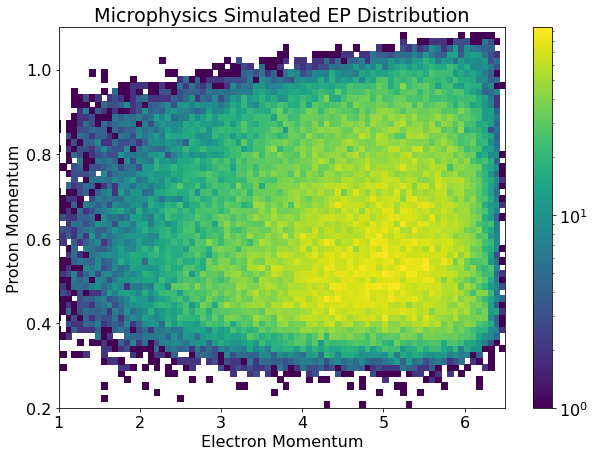
\includegraphics[width=.9\textwidth,trim={0 0 0 0},clip]{pictures/milestoneR2/gemc1.png}
        %\caption{(a)}
        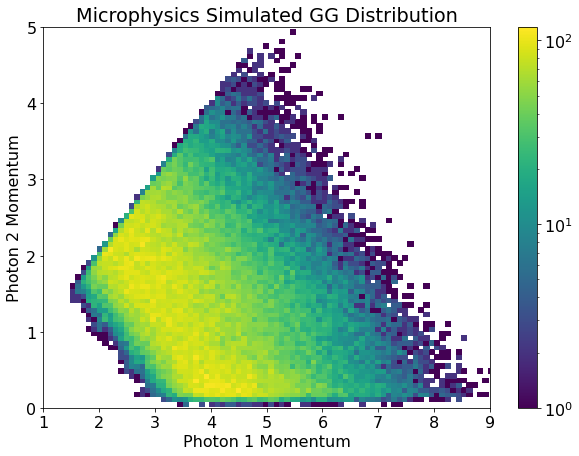
\includegraphics[width=.9\textwidth,trim={0 0 0 0},clip]{pictures/milestoneR2/gemc2.png}
        %\caption{(c)}
    \end{minipage}%
    \begin{minipage}{0.4\textwidth}
    Feature Distribution: NFlow Generated
        \centering
        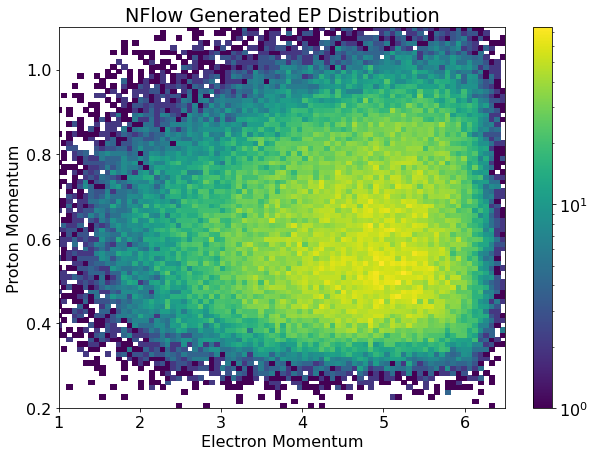
\includegraphics[width=.9\textwidth,trim={0 0 0 0},clip]{pictures/milestoneR2/nflow1.png}
        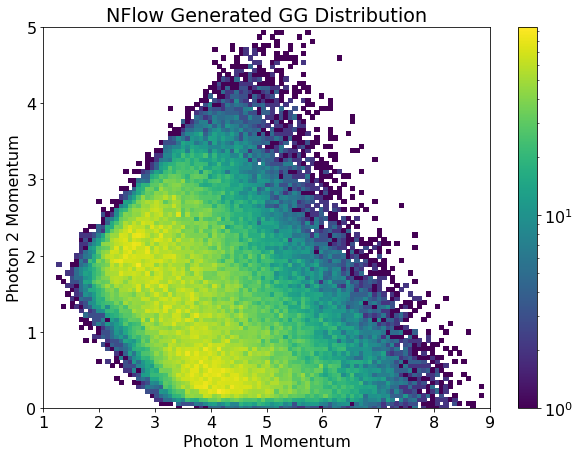
\includegraphics[width=.9\textwidth,trim={0 0 0 0},clip]{pictures/milestoneR2/nflow2.png}
    \end{minipage}
    \caption{\textbf{Left}: 2D distributions of the physics data $\mathbf{x_1}$. \textbf{Right}: 2D distributions of the data generated from the MAF $\mathbf{x_2}$.}
    \label{fig:a}
\end{figure}

\begin{figure}[!ht]
    \centering
    \begin{minipage}{1\textwidth}
    Feature Distribution: Physics Data
        \centering
        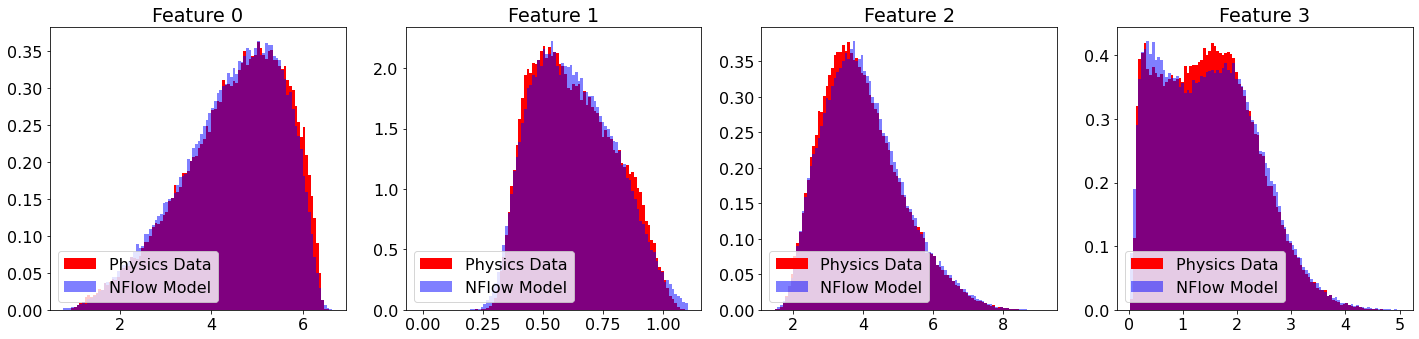
\includegraphics[width=.9\textwidth,trim={0 0 0 0},clip]{pictures/milestoneR2/comp1.png}
        %\caption{(a)}
        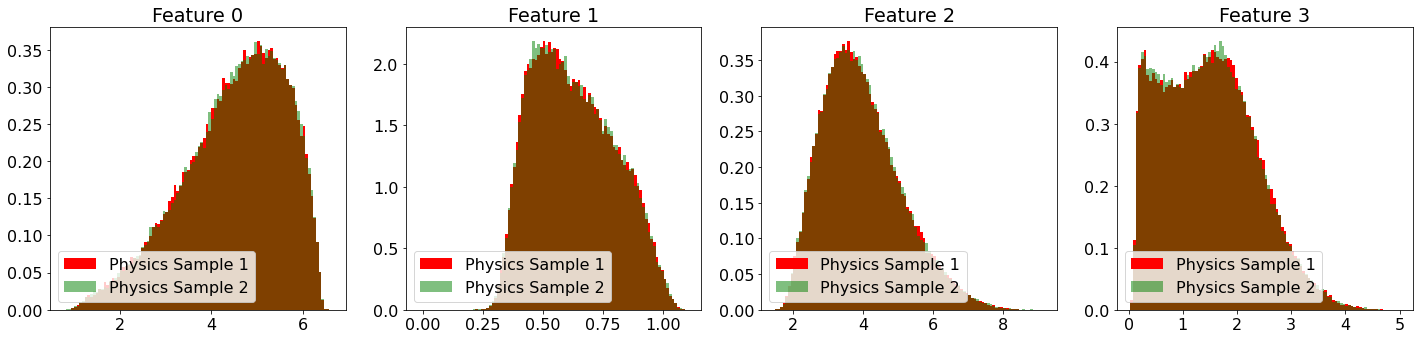
\includegraphics[width=.9\textwidth,trim={0 0 0 0},clip]{pictures/milestoneR2/comp2.png}
        %\caption{(c)}
    \end{minipage}%
    \caption{\textbf{Top}: Distributions of each feature in $\mathbf{x_1}$ (labeled as `Physics Data') and $\mathbf{x_2}$ (labeled as `NFlow Model'). \textbf{Bottom}: Comparison of distributions of each feature in $\mathbf{x_1}$ (labeled as `Physics Sample 1') and $\mathbf{x_1'}$ (labeled as `Physics Sample 2'). See Table 1 for EMD and KLD values.}
    \label{fig:b}
\end{figure}


\begin{center}
\begin{table}[ht]
\caption{EMD and KLD Values from Fig. ~\ref{fig:b}}
\centering
\begin{tabular}{ |p{2.5cm}||p{1.4cm}|p{1.4cm}|p{1.4cm} |p{1.4cm}| }

 %\hline
 %\multicolumn{5}{|c|}{Values of EMD and KLD for Fig.~\ref{fig:b}} \\ 
 \hline
%Quantity &  \multicolumn{4}{|c|}{Feature Number} \\ 
\textbf{Quantity} & \textbf{Feature 0} & \textbf{Feature 1} & \textbf{Feature 2} & \textbf{Feature 3} \\
 \hline                                             
%\multirow{2}{4em}{EMD}  & 0.0671 & 0.0048 & 0.0469 & 0.03533\\ 
EMD - NFlow  & 0.0671 & 0.0048 & 0.0469 & 0.0353\\ 
EMD - Sample & 0.0111 & 0.0006 & 0.0148 & 0.0038\\ 

\hhline{|=|=|=|=|=|}
%\multirow{2}{4em}{KLD} & $\infty$ & 0.0748 & 0.07969 & $\infty$\\ 
KLD- NFlow & $\infty$ & 0.0748 & 0.07969 & $\infty$\\ 
KLD - Sample & 0.0721 & 0.0730 & 0.07962 & 0.3973 \\ 

 \hline
\end{tabular}
\end{table}
\end{center}

\iffalse
\begin{center}
\begin{tabular}{c c c c c c }
Quantity & F0 & F1 & F2 & F3  \\
\hline
NFlow EMD & 0.0671 & 0.0048 & 0.0469 & 0.0353 \\ 
Sample EMD & 0.0111 & 0.0006 & 0.0148 & 0.0038 \\
NFlow KLD & $\infty$ & 0.0748 & 0.07969 & $\infty$\\  
Sample KLD & 0.0721 & 0.0730 & 0.07962 & 0.3973\\ 
\end{tabular}
\end{center}
\fi

Examining Table 1, we can see that our model is performing reasonably, with room to improve. Note that we did not restrict the flow to generate data only in regions of phase space where data exists for the physics set, so it is possible to have infinite divergence for the KLD value, although it is not helpful. Where it is well defined, we see very similar values between the MAF generated dataset $\mathbf{x_2}$ and the comparison dataset $\mathbf{x_1'}$. The EMD is defined at all times in our process, and so it is very useful, and indicates a somewhat worse agreement between our model and a perfect replica of the distribution. 


\begin{figure}[!ht]
    \centering
    \begin{minipage}{.25\textwidth}
    
        \centering
        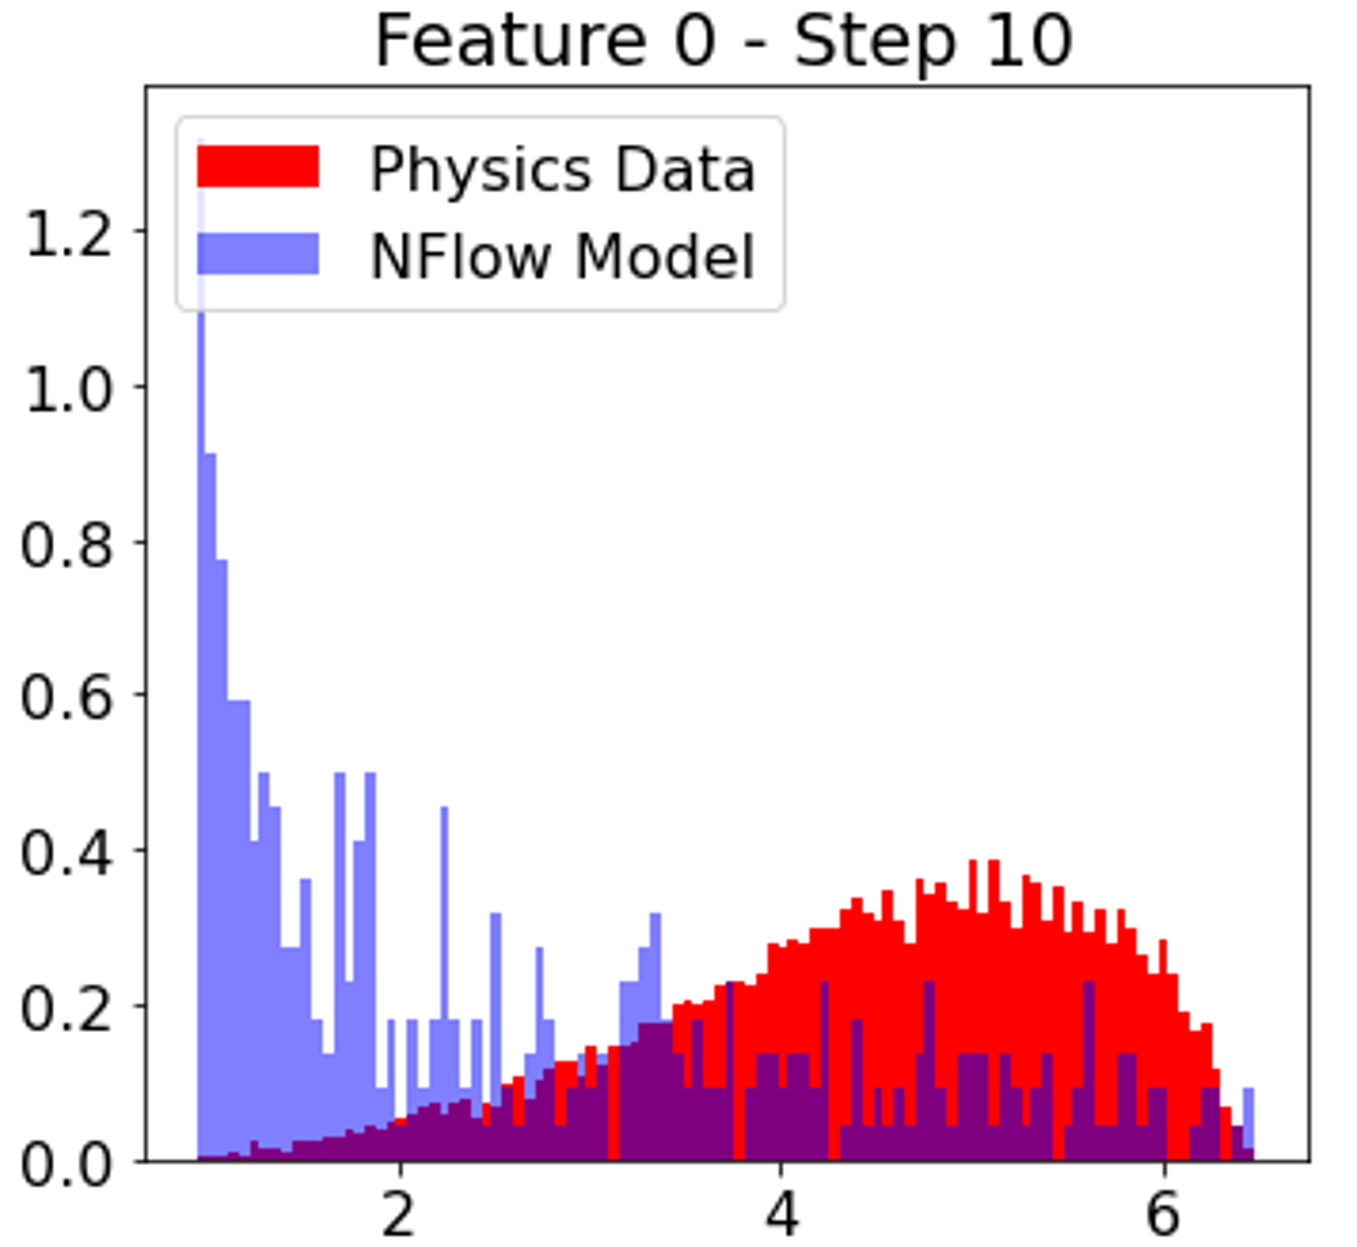
\includegraphics[width=.9\textwidth,trim={0 0 0 0},clip]{pictures/milestoneR2/steps/s10.png}
        %\caption{(a)}
        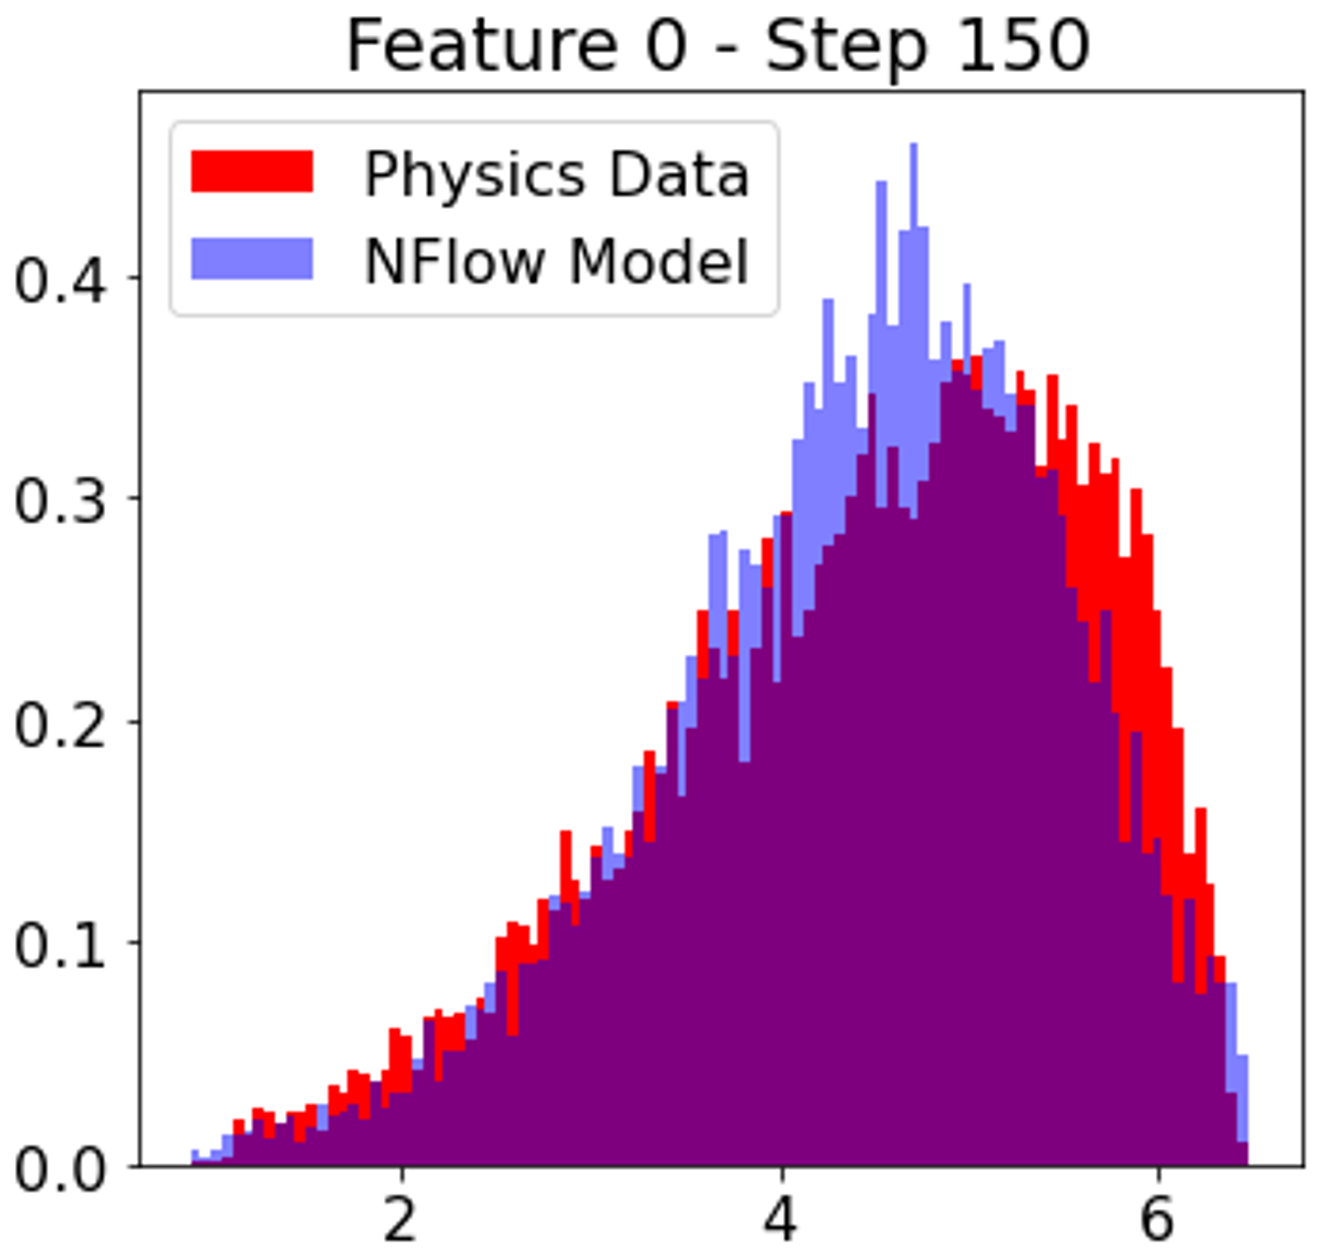
\includegraphics[width=.9\textwidth,trim={0 0 0 0},clip]{pictures/milestoneR2/steps/s150.png}
        %\caption{(c)}
    \end{minipage}%
    \begin{minipage}{0.25\textwidth}
    
        \centering
        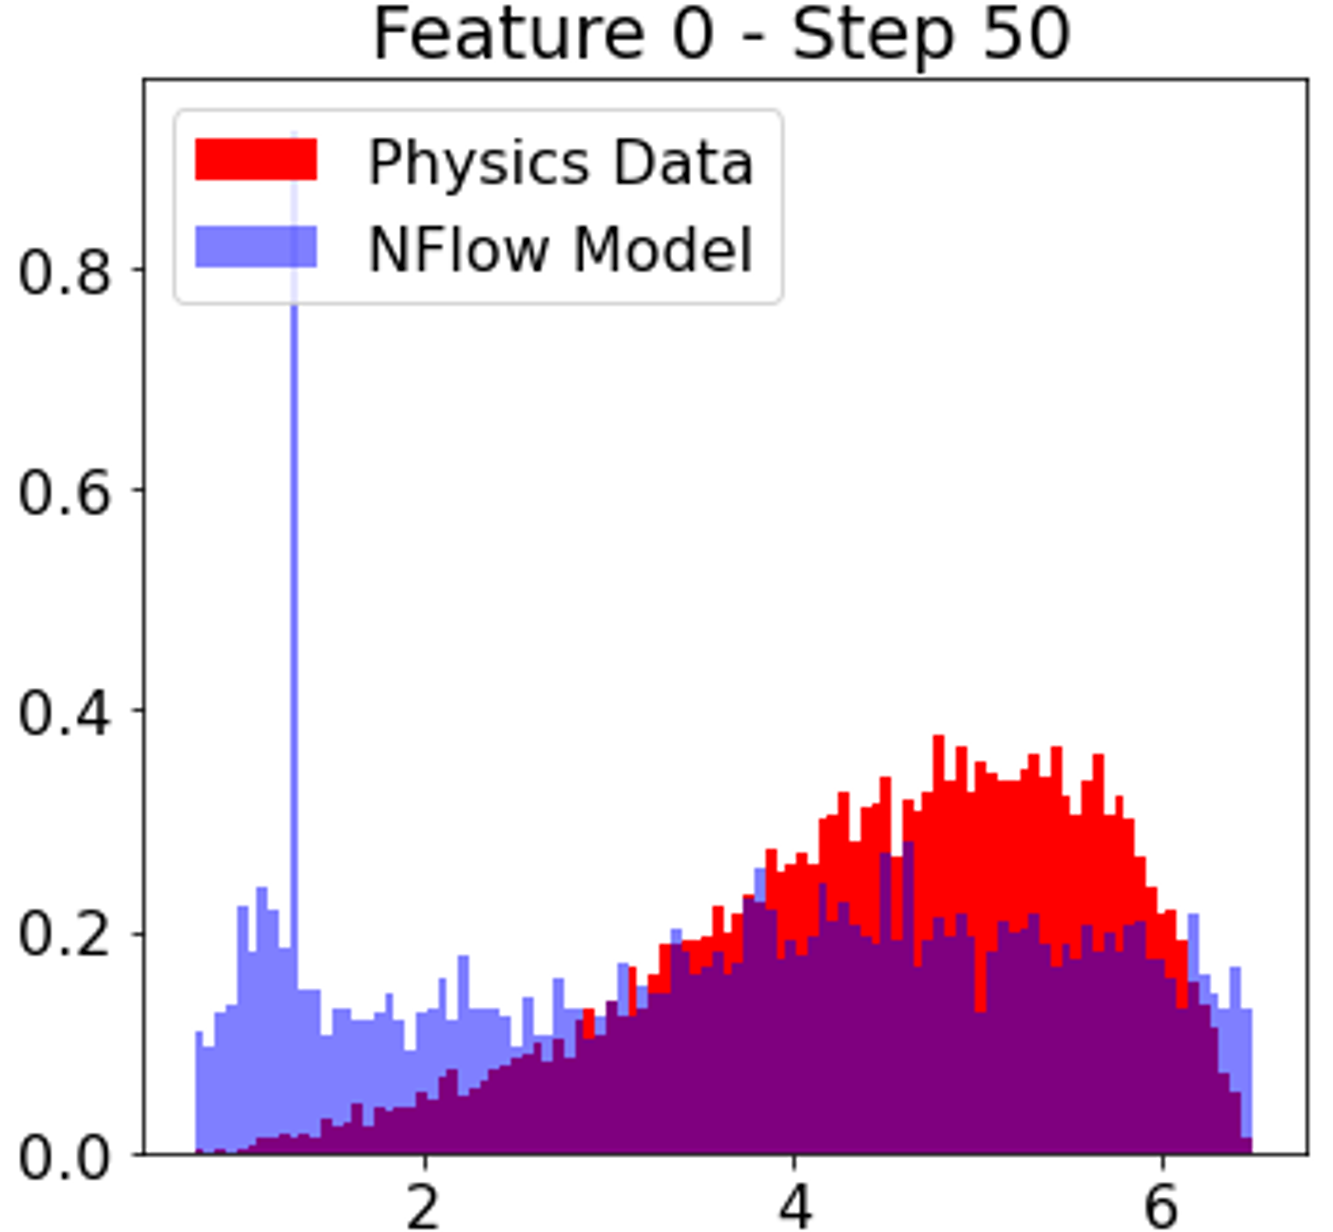
\includegraphics[width=.9\textwidth,trim={0 0 0 0},clip]{pictures/milestoneR2/steps/s50.png}
        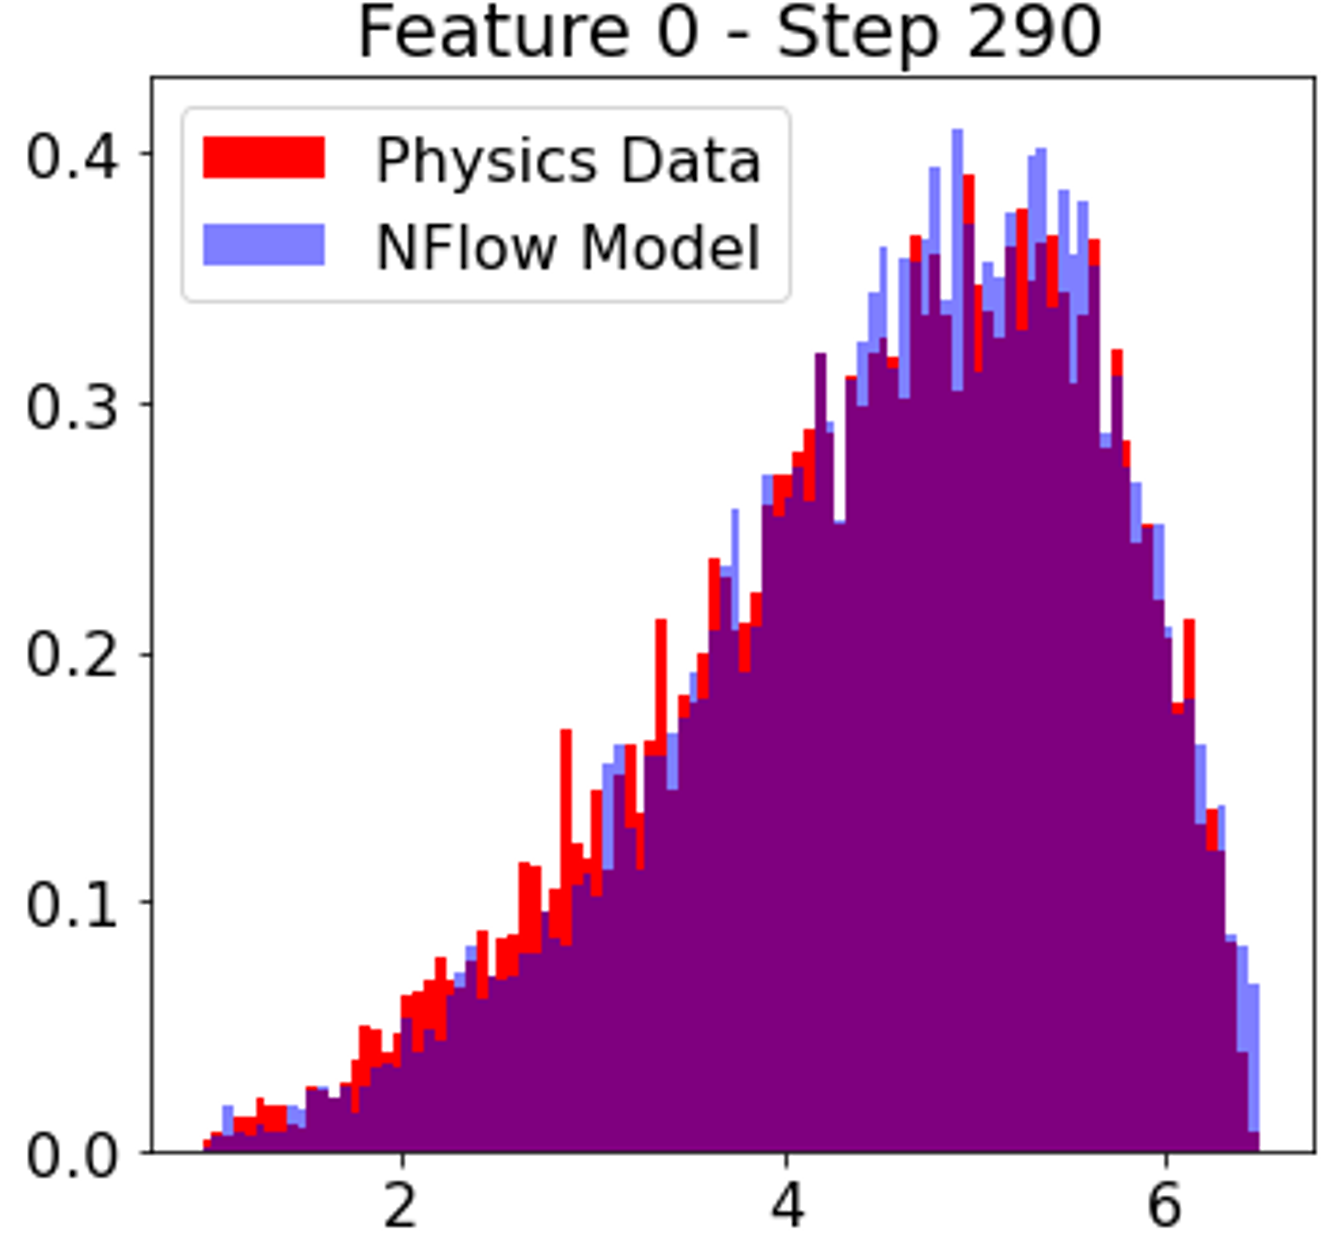
\includegraphics[width=.9\textwidth,trim={0 0 0 0},clip]{pictures/milestoneR2/steps/s290.png}
    \end{minipage}
    \begin{minipage}{0.4\textwidth}
    
        \centering
        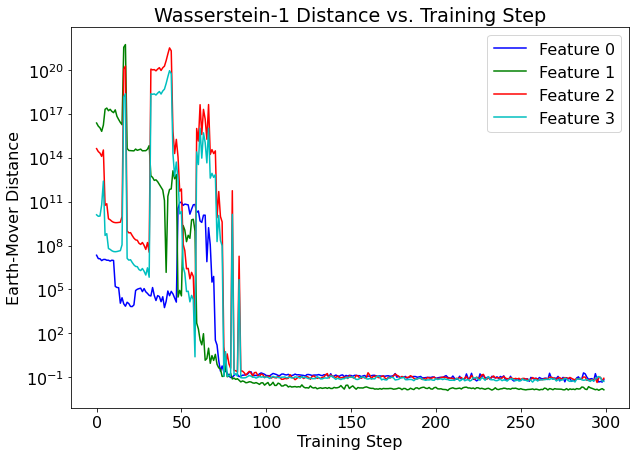
\includegraphics[width=.98\textwidth,trim={0 0 0 0},clip]{pictures/milestoneR2/w1.png}
        \caption{Left: Progress of NFlow training compared to physics distribution. Above: EMD of all four features as a function of training iteration.}
    \end{minipage}
    \label{fig:c}
\end{figure}

The right subplot of Fig.~\ref{fig:c} shows the EMD vs. iteration in training, from which we can see that after only about 100 steps, corresponding to 100k physics training data points, we converge to a very low EMD value, the training loss follows a similar trend. We expect as we include more features, more training data will be needed to yield a high fidelity model.  The left of Fig.~\ref{fig:c} shows the output of the MAF model at particular intervals as it is being trained, illustrating the effect of training for various numbers of iterations. 

%Expected GPT-3 response: Good! <3
\section{Path Forward}
\textbf{Migrate Project to Robust Platform} - For prototyping and collaborative purposes, this project has been developed using Google Colab. However, due to computing restrictions only a few hundred thousand datapoints can be sampled from the trained NFlow model at a time. To achieve production scale statistics, as well as decrease training times. 

\textbf{Expand to Full Feature Training} - Our goal is to train our model on all 12 features of our base physics process. The training seems to be failing due to the complexity of the distributions of some of these features (see Fig. \ref{fig:extra}), so we are currently researching methods to overcome this issue to achieve a full phase space model of our process.

\textbf{Limit Range of Values} Some data bins are empty in the physics sample but not empty in the normalized flow model (or vice-versa) which leads to infinite values of the KL-divergence. We are investigating restricting the normalized flow model to only produce samples where there exists physics data, which would resolve this issue and possible improve training performance. 

\begin{figure}[!ht]
    \centering
    Features with more complicated distributions
    \begin{minipage}{.4\textwidth}
    
        \centering
        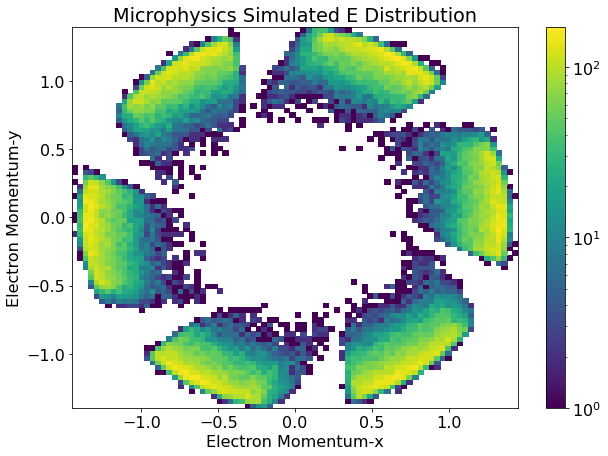
\includegraphics[width=.9\textwidth,trim={0 0 0 .875cm},clip]{pictures/milestoneR2/pxpy/epxpy.png}
        %\caption{(a)}
        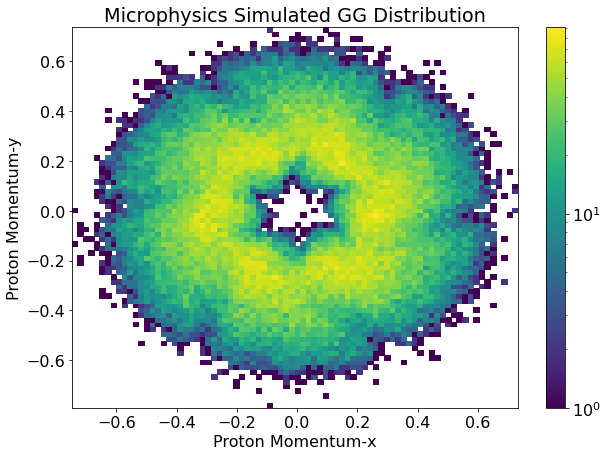
\includegraphics[width=.9\textwidth,trim={0 0 0 .875cm},clip]{pictures/milestoneR2/pxpy/ppxpy.png}
        %\caption{(c)}
    \end{minipage}%
    \begin{minipage}{0.4\textwidth}
    
        \centering
        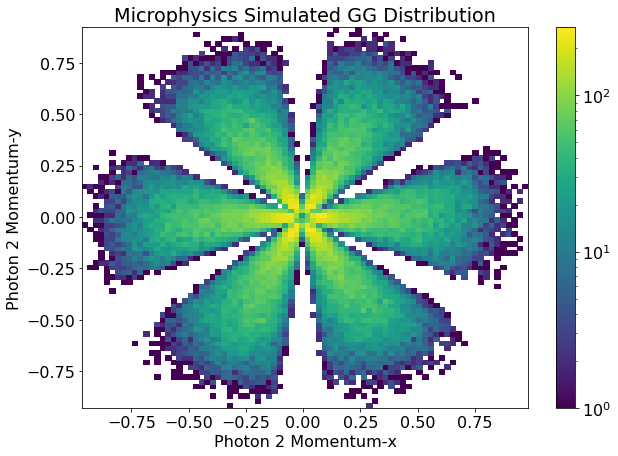
\includegraphics[width=.9\textwidth,trim={0 0 0 .875cm},clip]{pictures/milestoneR2/pxpy/g2pxpy.png}
        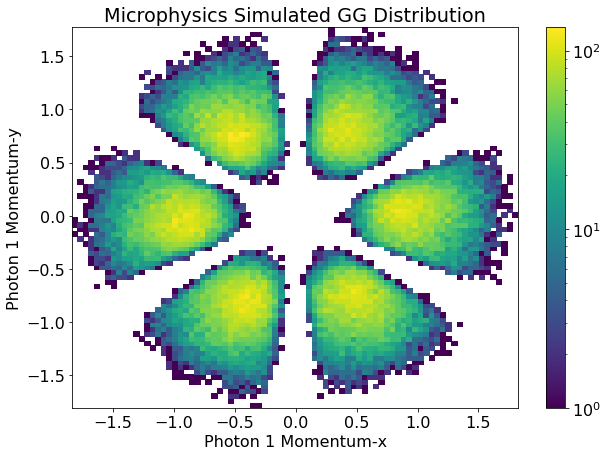
\includegraphics[width=.9\textwidth,trim={0 0 0 .875cm},clip]{pictures/milestoneR2/pxpy/gpxpy.png}
    \end{minipage}
    \caption{Nontrivial feature distributions from physics data that are yet to be modeled successfully by the NFlow model.}
    \label{fig:extra}
\end{figure}


\iffalse
Path forward:\\
Utilization of "z" distribution to train prior distribution\\
Expand to full feature representation learning\\
\fi


\iffalse
Parameters for best run:

prior = TransformedDistribution(Uniform(torch.zeros(2), torch.ones(2)), SigmoidTransform().inv) # Logistic distribution
#prior = MultivariateNormal(torch.zeros(2), torch.eye(2))
# NICE
flows = [AffineHalfFlow(dim=2, parity=i%2, scale=False) for i in range(12)]
#print(flows)
flows.append(AffineConstantFlow(dim=2, shift=False))
#print(flows)


# construct the model
model = NormalizingFlowModel(prior, flows)

optimizer = optim.Adam(model.parameters(), lr=5e-4, weight\_decay=1e-9)
for k in range(5000):
    sampleDict = xz.sample(1000)
    

 Path forward:
 working just on google colab, we quickly run into computing performance issues
 \fi